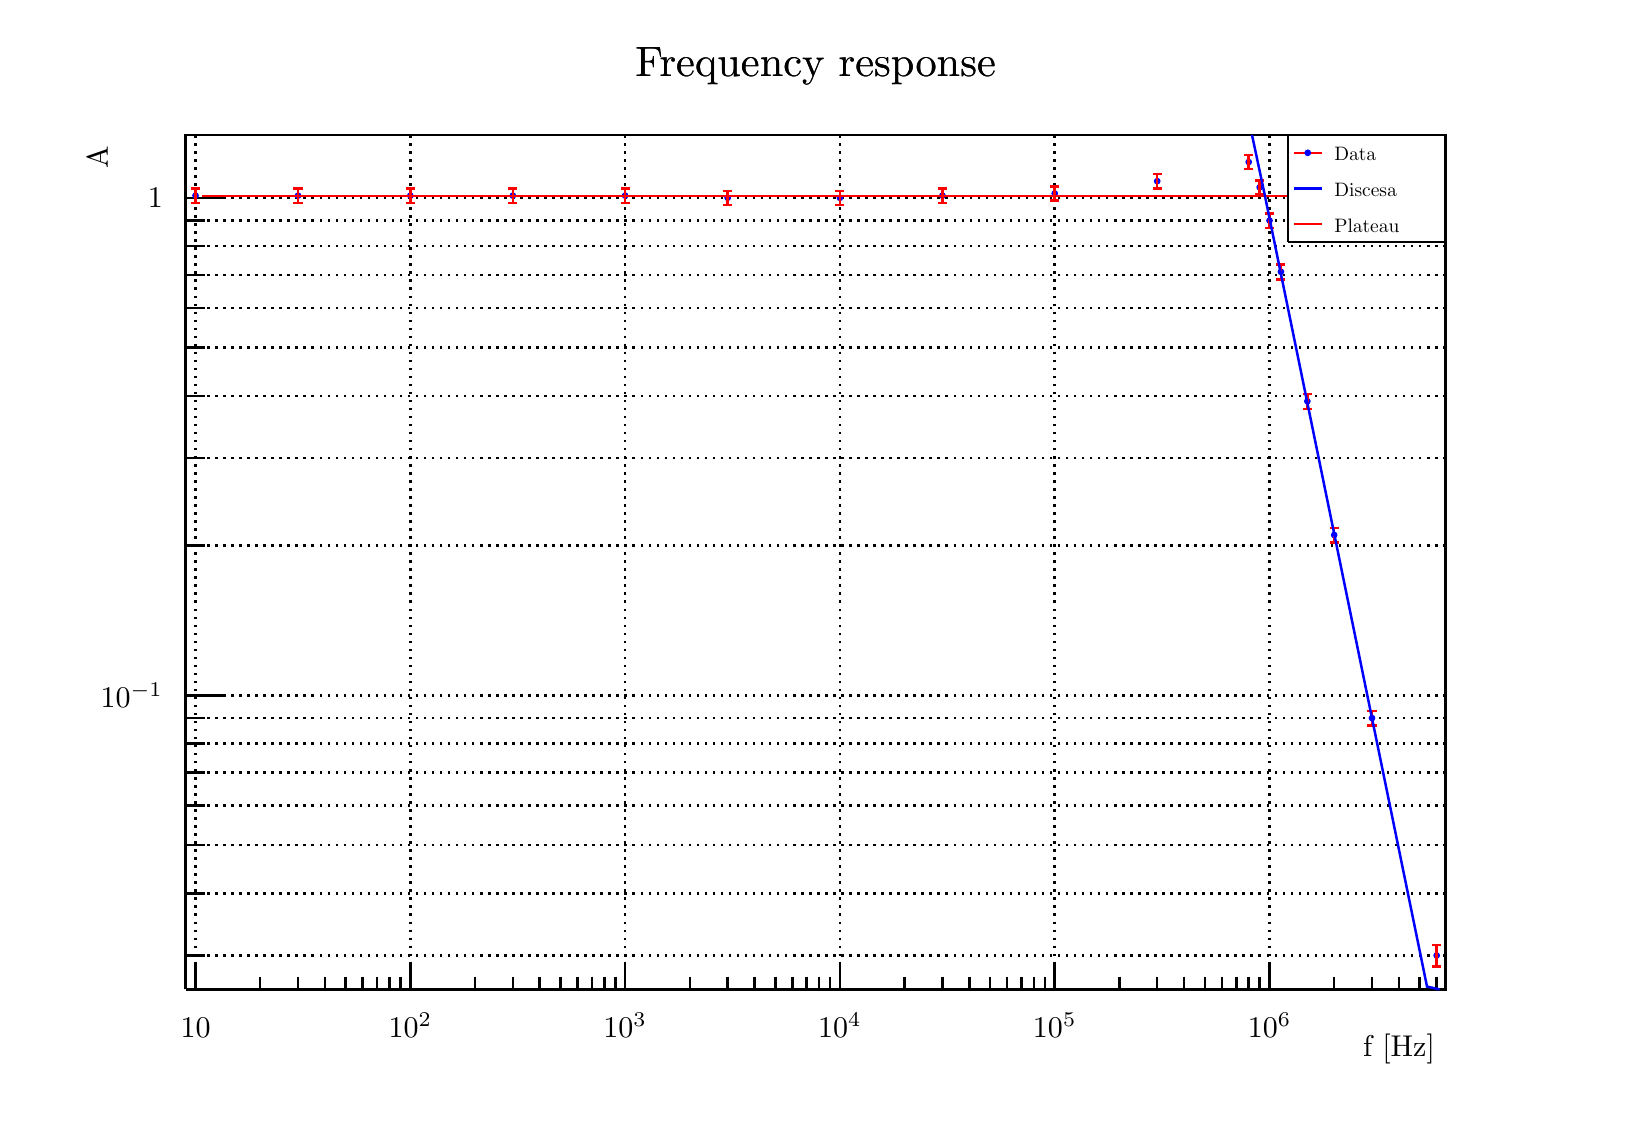
\begin{tikzpicture}
\pgfdeclareplotmark{cross} {
\pgfpathmoveto{\pgfpoint{-0.3\pgfplotmarksize}{\pgfplotmarksize}}
\pgfpathlineto{\pgfpoint{+0.3\pgfplotmarksize}{\pgfplotmarksize}}
\pgfpathlineto{\pgfpoint{+0.3\pgfplotmarksize}{0.3\pgfplotmarksize}}
\pgfpathlineto{\pgfpoint{+1\pgfplotmarksize}{0.3\pgfplotmarksize}}
\pgfpathlineto{\pgfpoint{+1\pgfplotmarksize}{-0.3\pgfplotmarksize}}
\pgfpathlineto{\pgfpoint{+0.3\pgfplotmarksize}{-0.3\pgfplotmarksize}}
\pgfpathlineto{\pgfpoint{+0.3\pgfplotmarksize}{-1.\pgfplotmarksize}}
\pgfpathlineto{\pgfpoint{-0.3\pgfplotmarksize}{-1.\pgfplotmarksize}}
\pgfpathlineto{\pgfpoint{-0.3\pgfplotmarksize}{-0.3\pgfplotmarksize}}
\pgfpathlineto{\pgfpoint{-1.\pgfplotmarksize}{-0.3\pgfplotmarksize}}
\pgfpathlineto{\pgfpoint{-1.\pgfplotmarksize}{0.3\pgfplotmarksize}}
\pgfpathlineto{\pgfpoint{-0.3\pgfplotmarksize}{0.3\pgfplotmarksize}}
\pgfpathclose
\pgfusepathqstroke
}
\pgfdeclareplotmark{cross*} {
\pgfpathmoveto{\pgfpoint{-0.3\pgfplotmarksize}{\pgfplotmarksize}}
\pgfpathlineto{\pgfpoint{+0.3\pgfplotmarksize}{\pgfplotmarksize}}
\pgfpathlineto{\pgfpoint{+0.3\pgfplotmarksize}{0.3\pgfplotmarksize}}
\pgfpathlineto{\pgfpoint{+1\pgfplotmarksize}{0.3\pgfplotmarksize}}
\pgfpathlineto{\pgfpoint{+1\pgfplotmarksize}{-0.3\pgfplotmarksize}}
\pgfpathlineto{\pgfpoint{+0.3\pgfplotmarksize}{-0.3\pgfplotmarksize}}
\pgfpathlineto{\pgfpoint{+0.3\pgfplotmarksize}{-1.\pgfplotmarksize}}
\pgfpathlineto{\pgfpoint{-0.3\pgfplotmarksize}{-1.\pgfplotmarksize}}
\pgfpathlineto{\pgfpoint{-0.3\pgfplotmarksize}{-0.3\pgfplotmarksize}}
\pgfpathlineto{\pgfpoint{-1.\pgfplotmarksize}{-0.3\pgfplotmarksize}}
\pgfpathlineto{\pgfpoint{-1.\pgfplotmarksize}{0.3\pgfplotmarksize}}
\pgfpathlineto{\pgfpoint{-0.3\pgfplotmarksize}{0.3\pgfplotmarksize}}
\pgfpathclose
\pgfusepathqfillstroke
}
\pgfdeclareplotmark{newstar} {
\pgfpathmoveto{\pgfqpoint{0pt}{\pgfplotmarksize}}
\pgfpathlineto{\pgfqpointpolar{44}{0.5\pgfplotmarksize}}
\pgfpathlineto{\pgfqpointpolar{18}{\pgfplotmarksize}}
\pgfpathlineto{\pgfqpointpolar{-20}{0.5\pgfplotmarksize}}
\pgfpathlineto{\pgfqpointpolar{-54}{\pgfplotmarksize}}
\pgfpathlineto{\pgfqpointpolar{-90}{0.5\pgfplotmarksize}}
\pgfpathlineto{\pgfqpointpolar{234}{\pgfplotmarksize}}
\pgfpathlineto{\pgfqpointpolar{198}{0.5\pgfplotmarksize}}
\pgfpathlineto{\pgfqpointpolar{162}{\pgfplotmarksize}}
\pgfpathlineto{\pgfqpointpolar{134}{0.5\pgfplotmarksize}}
\pgfpathclose
\pgfusepathqstroke
}
\pgfdeclareplotmark{newstar*} {
\pgfpathmoveto{\pgfqpoint{0pt}{\pgfplotmarksize}}
\pgfpathlineto{\pgfqpointpolar{44}{0.5\pgfplotmarksize}}
\pgfpathlineto{\pgfqpointpolar{18}{\pgfplotmarksize}}
\pgfpathlineto{\pgfqpointpolar{-20}{0.5\pgfplotmarksize}}
\pgfpathlineto{\pgfqpointpolar{-54}{\pgfplotmarksize}}
\pgfpathlineto{\pgfqpointpolar{-90}{0.5\pgfplotmarksize}}
\pgfpathlineto{\pgfqpointpolar{234}{\pgfplotmarksize}}
\pgfpathlineto{\pgfqpointpolar{198}{0.5\pgfplotmarksize}}
\pgfpathlineto{\pgfqpointpolar{162}{\pgfplotmarksize}}
\pgfpathlineto{\pgfqpointpolar{134}{0.5\pgfplotmarksize}}
\pgfpathclose
\pgfusepathqfillstroke
}
\definecolor{c}{rgb}{1,1,1};
\draw [color=c, fill=c] (0,0) rectangle (20,13.5632);
\draw [color=c, fill=c] (2,1.35632) rectangle (18,12.2069);
\definecolor{c}{rgb}{0,0,0};
\draw [c,line width=0.9] (2,1.35632) -- (2,12.2069) -- (18,12.2069) -- (18,1.35632) -- (2,1.35632);
\draw [c,line width=0.9] (2,1.35632) -- (18,1.35632);
\draw [c,dotted,line width=0.9] (2.12482,12.2069) -- (2.12482,1.35632);
\draw [c,dotted,line width=0.9] (4.85273,12.2069) -- (4.85273,1.35632);
\draw [c,dotted,line width=0.9] (7.58064,12.2069) -- (7.58064,1.35632);
\draw [c,dotted,line width=0.9] (10.3085,12.2069) -- (10.3085,1.35632);
\draw [c,dotted,line width=0.9] (13.0365,12.2069) -- (13.0365,1.35632);
\draw [c,dotted,line width=0.9] (15.7644,12.2069) -- (15.7644,1.35632);
\draw [c,line width=0.9] (2,1.35632) -- (2,12.2069);
\draw [c,dotted,line width=0.9] (18,1.78746) -- (2,1.78746);
\draw [c,dotted,line width=0.9] (18,2.57687) -- (2,2.57687);
\draw [c,dotted,line width=0.9] (18,3.18919) -- (2,3.18919);
\draw [c,dotted,line width=0.9] (18,3.68949) -- (2,3.68949);
\draw [c,dotted,line width=0.9] (18,4.11248) -- (2,4.11248);
\draw [c,dotted,line width=0.9] (18,4.4789) -- (2,4.4789);
\draw [c,dotted,line width=0.9] (18,4.8021) -- (2,4.8021);
\draw [c,dotted,line width=0.9] (18,5.09122) -- (2,5.09122);
\draw [c,dotted,line width=0.9] (18,6.99325) -- (2,6.99325);
\draw [c,dotted,line width=0.9] (18,8.10586) -- (2,8.10586);
\draw [c,dotted,line width=0.9] (18,8.89528) -- (2,8.89528);
\draw [c,dotted,line width=0.9] (18,9.50759) -- (2,9.50759);
\draw [c,dotted,line width=0.9] (18,10.0079) -- (2,10.0079);
\draw [c,dotted,line width=0.9] (18,10.4309) -- (2,10.4309);
\draw [c,dotted,line width=0.9] (18,10.7973) -- (2,10.7973);
\draw [c,dotted,line width=0.9] (18,11.1205) -- (2,11.1205);
\draw [c,dotted,line width=0.9] (18,11.4096) -- (2,11.4096);
\draw [c,line width=0.9] (2,1.35632) -- (18,1.35632);
\draw [anchor= east] (18,0.596782) node[scale=1.08496, color=c, rotate=0]{f [Hz]};
\draw [c,line width=0.9] (2.12482,1.68184) -- (2.12482,1.35632);
\draw [anchor=base] (2.12482,0.742586) node[scale=1.08496, color=c, rotate=0]{10};
\draw [c,line width=0.9] (2.946,1.51908) -- (2.946,1.35632);
\draw [c,line width=0.9] (3.42636,1.51908) -- (3.42636,1.35632);
\draw [c,line width=0.9] (3.76718,1.51908) -- (3.76718,1.35632);
\draw [c,line width=0.9] (4.03155,1.51908) -- (4.03155,1.35632);
\draw [c,line width=0.9] (4.24754,1.51908) -- (4.24754,1.35632);
\draw [c,line width=0.9] (4.43017,1.51908) -- (4.43017,1.35632);
\draw [c,line width=0.9] (4.58837,1.51908) -- (4.58837,1.35632);
\draw [c,line width=0.9] (4.72791,1.51908) -- (4.72791,1.35632);
\draw [c,line width=0.9] (4.85273,1.68184) -- (4.85273,1.35632);
\draw [anchor=base] (4.85273,0.742586) node[scale=1.08496, color=c, rotate=0]{$10^{2}$};
\draw [c,line width=0.9] (5.67391,1.51908) -- (5.67391,1.35632);
\draw [c,line width=0.9] (6.15427,1.51908) -- (6.15427,1.35632);
\draw [c,line width=0.9] (6.49509,1.51908) -- (6.49509,1.35632);
\draw [c,line width=0.9] (6.75945,1.51908) -- (6.75945,1.35632);
\draw [c,line width=0.9] (6.97545,1.51908) -- (6.97545,1.35632);
\draw [c,line width=0.9] (7.15808,1.51908) -- (7.15808,1.35632);
\draw [c,line width=0.9] (7.31627,1.51908) -- (7.31627,1.35632);
\draw [c,line width=0.9] (7.45581,1.51908) -- (7.45581,1.35632);
\draw [c,line width=0.9] (7.58064,1.68184) -- (7.58064,1.35632);
\draw [anchor=base] (7.58064,0.742586) node[scale=1.08496, color=c, rotate=0]{$10^{3}$};
\draw [c,line width=0.9] (8.40182,1.51908) -- (8.40182,1.35632);
\draw [c,line width=0.9] (8.88218,1.51908) -- (8.88218,1.35632);
\draw [c,line width=0.9] (9.223,1.51908) -- (9.223,1.35632);
\draw [c,line width=0.9] (9.48736,1.51908) -- (9.48736,1.35632);
\draw [c,line width=0.9] (9.70336,1.51908) -- (9.70336,1.35632);
\draw [c,line width=0.9] (9.88599,1.51908) -- (9.88599,1.35632);
\draw [c,line width=0.9] (10.0442,1.51908) -- (10.0442,1.35632);
\draw [c,line width=0.9] (10.1837,1.51908) -- (10.1837,1.35632);
\draw [c,line width=0.9] (10.3085,1.68184) -- (10.3085,1.35632);
\draw [anchor=base] (10.3085,0.742586) node[scale=1.08496, color=c, rotate=0]{$10^{4}$};
\draw [c,line width=0.9] (11.1297,1.51908) -- (11.1297,1.35632);
\draw [c,line width=0.9] (11.6101,1.51908) -- (11.6101,1.35632);
\draw [c,line width=0.9] (11.9509,1.51908) -- (11.9509,1.35632);
\draw [c,line width=0.9] (12.2153,1.51908) -- (12.2153,1.35632);
\draw [c,line width=0.9] (12.4313,1.51908) -- (12.4313,1.35632);
\draw [c,line width=0.9] (12.6139,1.51908) -- (12.6139,1.35632);
\draw [c,line width=0.9] (12.7721,1.51908) -- (12.7721,1.35632);
\draw [c,line width=0.9] (12.9116,1.51908) -- (12.9116,1.35632);
\draw [c,line width=0.9] (13.0365,1.68184) -- (13.0365,1.35632);
\draw [anchor=base] (13.0365,0.742586) node[scale=1.08496, color=c, rotate=0]{$10^{5}$};
\draw [c,line width=0.9] (13.8576,1.51908) -- (13.8576,1.35632);
\draw [c,line width=0.9] (14.338,1.51908) -- (14.338,1.35632);
\draw [c,line width=0.9] (14.6788,1.51908) -- (14.6788,1.35632);
\draw [c,line width=0.9] (14.9432,1.51908) -- (14.9432,1.35632);
\draw [c,line width=0.9] (15.1592,1.51908) -- (15.1592,1.35632);
\draw [c,line width=0.9] (15.3418,1.51908) -- (15.3418,1.35632);
\draw [c,line width=0.9] (15.5,1.51908) -- (15.5,1.35632);
\draw [c,line width=0.9] (15.6395,1.51908) -- (15.6395,1.35632);
\draw [c,line width=0.9] (15.7644,1.68184) -- (15.7644,1.35632);
\draw [anchor=base] (15.7644,0.742586) node[scale=1.08496, color=c, rotate=0]{$10^{6}$};
\draw [c,line width=0.9] (16.5855,1.51908) -- (16.5855,1.35632);
\draw [c,line width=0.9] (17.0659,1.51908) -- (17.0659,1.35632);
\draw [c,line width=0.9] (17.4067,1.51908) -- (17.4067,1.35632);
\draw [c,line width=0.9] (17.6711,1.51908) -- (17.6711,1.35632);
\draw [c,line width=0.9] (17.8871,1.51908) -- (17.8871,1.35632);
\draw [c,line width=0.9] (2,1.35632) -- (2,12.2069);
\draw [anchor= east] (0.88,12.2069) node[scale=1.08496, color=c, rotate=90]{A};
\draw [c,line width=0.9] (2.24,1.78746) -- (2,1.78746);
\draw [c,line width=0.9] (2.24,2.57687) -- (2,2.57687);
\draw [c,line width=0.9] (2.24,3.18919) -- (2,3.18919);
\draw [c,line width=0.9] (2.24,3.68949) -- (2,3.68949);
\draw [c,line width=0.9] (2.24,4.11248) -- (2,4.11248);
\draw [c,line width=0.9] (2.24,4.4789) -- (2,4.4789);
\draw [c,line width=0.9] (2.24,4.8021) -- (2,4.8021);
\draw [c,line width=0.9] (2.48,5.09122) -- (2,5.09122);
\draw [anchor= east] (1.844,5.09122) node[scale=1.08496, color=c, rotate=0]{$10^{-1}$};
\draw [c,line width=0.9] (2.24,6.99325) -- (2,6.99325);
\draw [c,line width=0.9] (2.24,8.10586) -- (2,8.10586);
\draw [c,line width=0.9] (2.24,8.89528) -- (2,8.89528);
\draw [c,line width=0.9] (2.24,9.50759) -- (2,9.50759);
\draw [c,line width=0.9] (2.24,10.0079) -- (2,10.0079);
\draw [c,line width=0.9] (2.24,10.4309) -- (2,10.4309);
\draw [c,line width=0.9] (2.24,10.7973) -- (2,10.7973);
\draw [c,line width=0.9] (2.24,11.1205) -- (2,11.1205);
\draw [c,line width=0.9] (2.48,11.4096) -- (2,11.4096);
\draw [anchor= east] (1.844,11.4096) node[scale=1.08496, color=c, rotate=0]{1};
\draw (10,13.0816) node[scale=1.5317, color=c, rotate=0]{Frequency response};
\definecolor{c}{rgb}{0,0,1};
\foreach \P in {(2.12482,11.4369), (3.42636,11.4369), (4.85273,11.4369), (6.15427,11.4369), (7.58064,11.4369), (8.88218,11.4096), (10.3085,11.4096), (11.6101,11.4369), (13.0365,11.464), (14.338,11.6208), (15.5,11.8638), (15.6395,11.5435),
 (15.7644,11.1205), (15.9092,10.4698), (16.2447,8.8258), (16.5855,7.12713), (17.0659,4.8021), (17.8871,1.78745)}{\draw[mark options={color=c,fill=c},mark size=1.681682pt,mark=*,mark size=1pt] plot coordinates {\P};}
\definecolor{c}{rgb}{1,0,0};
\draw [c,line width=0.9] (2.12482,11.4369) -- (2.12482,11.5259);
\draw [c,line width=0.9] (2.06735,11.5259) -- (2.18229,11.5259);
\draw [c,line width=0.9] (2.12482,11.4369) -- (2.12482,11.345);
\draw [c,line width=0.9] (2.06735,11.345) -- (2.18229,11.345);
\draw [c,line width=0.9] (3.42636,11.4369) -- (3.42636,11.5259);
\draw [c,line width=0.9] (3.36889,11.5259) -- (3.48384,11.5259);
\draw [c,line width=0.9] (3.42636,11.4369) -- (3.42636,11.345);
\draw [c,line width=0.9] (3.36889,11.345) -- (3.48384,11.345);
\draw [c,line width=0.9] (4.85273,11.4369) -- (4.85273,11.5259);
\draw [c,line width=0.9] (4.79526,11.5259) -- (4.9102,11.5259);
\draw [c,line width=0.9] (4.85273,11.4369) -- (4.85273,11.345);
\draw [c,line width=0.9] (4.79526,11.345) -- (4.9102,11.345);
\draw [c,line width=0.9] (6.15427,11.4369) -- (6.15427,11.5259);
\draw [c,line width=0.9] (6.0968,11.5259) -- (6.21174,11.5259);
\draw [c,line width=0.9] (6.15427,11.4369) -- (6.15427,11.345);
\draw [c,line width=0.9] (6.0968,11.345) -- (6.21174,11.345);
\draw [c,line width=0.9] (7.58064,11.4369) -- (7.58064,11.5259);
\draw [c,line width=0.9] (7.52317,11.5259) -- (7.63811,11.5259);
\draw [c,line width=0.9] (7.58064,11.4369) -- (7.58064,11.345);
\draw [c,line width=0.9] (7.52317,11.345) -- (7.63811,11.345);
\draw [c,line width=0.9] (8.88218,11.4096) -- (8.88218,11.4987);
\draw [c,line width=0.9] (8.82471,11.4987) -- (8.93965,11.4987);
\draw [c,line width=0.9] (8.88218,11.4096) -- (8.88218,11.3176);
\draw [c,line width=0.9] (8.82471,11.3176) -- (8.93965,11.3176);
\draw [c,line width=0.9] (10.3085,11.4096) -- (10.3085,11.4987);
\draw [c,line width=0.9] (10.2511,11.4987) -- (10.366,11.4987);
\draw [c,line width=0.9] (10.3085,11.4096) -- (10.3085,11.3176);
\draw [c,line width=0.9] (10.2511,11.3176) -- (10.366,11.3176);
\draw [c,line width=0.9] (11.6101,11.4369) -- (11.6101,11.5259);
\draw [c,line width=0.9] (11.5526,11.5259) -- (11.6676,11.5259);
\draw [c,line width=0.9] (11.6101,11.4369) -- (11.6101,11.345);
\draw [c,line width=0.9] (11.5526,11.345) -- (11.6676,11.345);
\draw [c,line width=0.9] (13.0365,11.464) -- (13.0365,11.5528);
\draw [c,line width=0.9] (12.979,11.5528) -- (13.0939,11.5528);
\draw [c,line width=0.9] (13.0365,11.464) -- (13.0365,11.3722);
\draw [c,line width=0.9] (12.979,11.3722) -- (13.0939,11.3722);
\draw [c,line width=0.9] (14.338,11.6208) -- (14.338,11.709);
\draw [c,line width=0.9] (14.2805,11.709) -- (14.3955,11.709);
\draw [c,line width=0.9] (14.338,11.6208) -- (14.338,11.5297);
\draw [c,line width=0.9] (14.2805,11.5297) -- (14.3955,11.5297);
\draw [c,line width=0.9] (15.5,11.8638) -- (15.5,11.9512);
\draw [c,line width=0.9] (15.4425,11.9512) -- (15.5575,11.9512);
\draw [c,line width=0.9] (15.5,11.8638) -- (15.5,11.7735);
\draw [c,line width=0.9] (15.4425,11.7735) -- (15.5575,11.7735);
\draw [c,line width=0.9] (15.6395,11.5435) -- (15.6395,11.632);
\draw [c,line width=0.9] (15.5821,11.632) -- (15.697,11.632);
\draw [c,line width=0.9] (15.6395,11.5435) -- (15.6395,11.452);
\draw [c,line width=0.9] (15.5821,11.452) -- (15.697,11.452);
\draw [c,line width=0.9] (15.7644,11.1205) -- (15.7644,11.2109);
\draw [c,line width=0.9] (15.7069,11.2109) -- (15.8218,11.2109);
\draw [c,line width=0.9] (15.7644,11.1205) -- (15.7644,11.027);
\draw [c,line width=0.9] (15.7069,11.027) -- (15.8218,11.027);
\draw [c,line width=0.9] (15.9092,10.4698) -- (15.9092,10.5644);
\draw [c,line width=0.9] (15.8517,10.5644) -- (15.9666,10.5644);
\draw [c,line width=0.9] (15.9092,10.4698) -- (15.9092,10.3719);
\draw [c,line width=0.9] (15.8517,10.3719) -- (15.9666,10.3719);
\draw [c,line width=0.9] (16.2447,8.8258) -- (16.2447,8.9185);
\draw [c,line width=0.9] (16.1873,8.9185) -- (16.3022,8.9185);
\draw [c,line width=0.9] (16.2447,8.8258) -- (16.2447,8.72985);
\draw [c,line width=0.9] (16.1873,8.72985) -- (16.3022,8.72985);
\draw [c,line width=0.9] (16.5855,7.12713) -- (16.5855,7.21856);
\draw [c,line width=0.9] (16.5281,7.21856) -- (16.643,7.21856);
\draw [c,line width=0.9] (16.5855,7.12713) -- (16.5855,7.03254);
\draw [c,line width=0.9] (16.5281,7.03254) -- (16.643,7.03254);
\draw [c,line width=0.9] (17.0659,4.8021) -- (17.0659,4.8925);
\draw [c,line width=0.9] (17.0084,4.8925) -- (17.1234,4.8925);
\draw [c,line width=0.9] (17.0659,4.8021) -- (17.0659,4.70862);
\draw [c,line width=0.9] (17.0084,4.70862) -- (17.1234,4.70862);
\draw [c,line width=0.9] (17.8871,1.78745) -- (17.8871,1.92248);
\draw [c,line width=0.9] (17.8296,1.92248) -- (17.9446,1.92248);
\draw [c,line width=0.9] (17.8871,1.78745) -- (17.8871,1.64544);
\draw [c,line width=0.9] (17.8296,1.64544) -- (17.9446,1.64544);
\draw [c,line width=0.9] (2.20686,11.4339) -- (2.36561,11.4339) -- (2.52436,11.4339) -- (2.68311,11.4339) -- (2.84186,11.4339) -- (3.00061,11.4339) -- (3.15937,11.4339) -- (3.31812,11.4339) -- (3.47687,11.4339) -- (3.63562,11.4339) --
 (3.79437,11.4339) -- (3.95312,11.4339) -- (4.11188,11.4339) -- (4.27063,11.4339) -- (4.42938,11.4339) -- (4.58813,11.4339) -- (4.74688,11.4339) -- (4.90564,11.4339) -- (5.06439,11.4339) -- (5.22314,11.4339) -- (5.38189,11.4339) -- (5.54064,11.4339)
 -- (5.69939,11.4339) -- (5.85815,11.4339) -- (6.0169,11.4339) -- (6.17565,11.4339) -- (6.3344,11.4339) -- (6.49315,11.4339) -- (6.65191,11.4339) -- (6.81066,11.4339) -- (6.96941,11.4339) -- (7.12816,11.4339) -- (7.28691,11.4339) -- (7.44566,11.4339)
 -- (7.60442,11.4339) -- (7.76317,11.4339) -- (7.92192,11.4339) -- (8.08067,11.4339) -- (8.23942,11.4339) -- (8.39817,11.4339) -- (8.55693,11.4339) -- (8.71568,11.4339) -- (8.87443,11.4339) -- (9.03318,11.4339) -- (9.19193,11.4339) --
 (9.35069,11.4339) -- (9.50944,11.4339) -- (9.66819,11.4339) -- (9.82694,11.4339) -- (9.98569,11.4339);
\draw [c,line width=0.9] (9.98569,11.4339) -- (10.1444,11.4339) -- (10.3032,11.4339) -- (10.4619,11.4339) -- (10.6207,11.4339) -- (10.7795,11.4339) -- (10.9382,11.4339) -- (11.097,11.4339) -- (11.2557,11.4339) -- (11.4145,11.4339) --
 (11.5732,11.4339) -- (11.732,11.4339) -- (11.8907,11.4339) -- (12.0495,11.4339) -- (12.2082,11.4339) -- (12.367,11.4339) -- (12.5257,11.4339) -- (12.6845,11.4339) -- (12.8432,11.4339) -- (13.002,11.4339) -- (13.1607,11.4339) -- (13.3195,11.4339) --
 (13.4782,11.4339) -- (13.637,11.4339) -- (13.7957,11.4339) -- (13.9545,11.4339) -- (14.1132,11.4339) -- (14.272,11.4339) -- (14.4307,11.4339) -- (14.5895,11.4339) -- (14.7482,11.4339) -- (14.907,11.4339) -- (15.0657,11.4339) -- (15.2245,11.4339) --
 (15.3833,11.4339) -- (15.542,11.4339) -- (15.7008,11.4339) -- (15.8595,11.4339) -- (16.0183,11.4339) -- (16.177,11.4339) -- (16.3358,11.4339) -- (16.4945,11.4339) -- (16.6533,11.4339) -- (16.812,11.4339) -- (16.9708,11.4339) -- (17.1295,11.4339) --
 (17.2883,11.4339) -- (17.447,11.4339) -- (17.6058,11.4339) -- (17.7645,11.4339);
\draw [c,line width=0.9] (17.7645,11.4339) -- (17.9233,11.4339);
\definecolor{c}{rgb}{0,0,1};
\draw [c,line width=0.9] (15.542,12.2069) -- (15.7008,11.4592) -- (15.8595,10.6848) -- (16.0183,9.91035) -- (16.177,9.13594) -- (16.3358,8.36153) -- (16.4945,7.58711) -- (16.6533,6.8127) -- (16.812,6.03829) -- (16.9708,5.26388) -- (17.1295,4.48946)
 -- (17.2883,3.71505) -- (17.447,2.94064) -- (17.6058,2.16623) -- (17.7645,1.39181) -- (17.9233,1.35632);
\definecolor{c}{rgb}{1,1,1};
\draw [color=c, fill=c] (16,10.8506) rectangle (18,12.2069);
\definecolor{c}{rgb}{0,0,0};
\draw [c,line width=0.9] (16,10.8506) -- (18,10.8506);
\draw [c,line width=0.9] (18,10.8506) -- (18,12.2069);
\draw [c,line width=0.9] (18,12.2069) -- (16,12.2069);
\draw [c,line width=0.9] (16,12.2069) -- (16,10.8506);
\draw [anchor=base west] (16.5,11.8791) node[scale=0.702031, color=c, rotate=0]{Data};
\definecolor{c}{rgb}{1,0,0};
\draw [c,line width=0.9] (16.075,11.9808) -- (16.425,11.9808);
\definecolor{c}{rgb}{0,0,1};
\foreach \P in {(16.25,11.9808)}{\draw[mark options={color=c,fill=c},mark size=1.681682pt,mark=*,mark size=1pt] plot coordinates {\P};}
\definecolor{c}{rgb}{0,0,0};
\draw [anchor=base west] (16.5,11.427) node[scale=0.702031, color=c, rotate=0]{Discesa};
\definecolor{c}{rgb}{0,0,1};
\draw [c,line width=0.9] (16.075,11.5287) -- (16.425,11.5287);
\definecolor{c}{rgb}{0,0,0};
\draw [anchor=base west] (16.5,10.9749) node[scale=0.702031, color=c, rotate=0]{Plateau};
\definecolor{c}{rgb}{1,0,0};
\draw [c,line width=0.9] (16.075,11.0766) -- (16.425,11.0766);
\definecolor{c}{rgb}{0,0,0};
\draw (10,13.0816) node[scale=1.5317, color=c, rotate=0]{Frequency response};
\end{tikzpicture}
